\begin{table}[t]
\footnotesize
\centering
\begin{tabular}{llccc}
\toprule
& Model & \# Forg. & \# Balanced Forg. & Acc.\\
\midrule
& BoW         &100,345 & \balancedbow & 64.0\\
\textit{MNLI} & BiLSTM      &76,270 & \balancedlstm  & 69.6\\
& BERT        &32,387 &  \balancedbert & 84.5\\
\midrule
& BoW         &73,478&71,116  & 81.1\\
\textit{QQP} & BiLSTM      &81,754 &76,634   & 84.3 \\
& BERT        &22,372 &20,498   & 91.3 \\
% OLD BALANCED_ALL_FORG:
%\midrule
%& BoW         &73,478&59,477  & 81.1\\
%\textit{QQP} & BiLSTM      &81,754 &68,130   & 84.3 \\
%& BERT        &22,372 &19,014   & 91.3 \\
\bottomrule
\end{tabular}
\caption{Number of ``forgettable'' examples (those that are forgotten at least once or never learned) during training along with the accuracy on the MNLI matched development sets and QQP.}
\label{tab:forg_stats}
\end{table}


\begin{table}
\setlength{\tabcolsep}{2.5pt}
\footnotesize
\centering
\begin{tabular}{l@{\hskip 0.04in}lccc}
\toprule
& \textbf{Train examples} & \textbf{HANS} & \textbf{MNLI} & \textbf{Avg.}  \\
\midrule
% \small{1} & All & 58.3 & \textbf{84.5} & 71.4        \\
% \small{1} & All & 57.9$_{\pm 1.2}$ & 84.4$_{\pm 0.1}$ &  71.2$_{\pm 0.6}$\\
& \textbf{\bertbase } (lines 1-16) \\
\small{1} & All & 63.1$_{\pm 1.2}$ & 84.5$_{\pm 0.1}$ &  73.8$_{\pm 1.0}$\\
\midrule
\small{2} & \fbert $_{(\balancedbert)}$   & 49.6$_{\pm 0.2}$                     & 37.9$_{\pm 1.3}$                         & 43.7$_{\pm 0.6}$ \\
\small{3} & \hspace{0.2cm} Random $_{(\balancedbert)}$ & 50.8$_{\pm 0.2}$                   & 74.7$_{\pm 0.4}$                         &  62.8$_{\pm 0.1}$ \\
\small{4} & \flstm $_{(\balancedlstm)}$ & 54.0$_{\pm 0.6}$                     & 66.7$_{\pm 0.9}$                         &  60.4$_{\pm 0.2}$  \\
\small{5} & \hspace{0.2cm} Random $_{(\balancedlstm)}$ & 51.3$_{\pm 0.6}$                   & 78.8$_{\pm 0.4}$                         &  65.1$_{\pm 0.3}$  \\
\small{6} & \fbow $_{(\balancedbow)}$    & 55.4$_{\pm 1.4}$                     & 68.2$_{\pm 0.8}$                         &  61.8$_{\pm 1.1}$  \\
\small{7} & \hspace{0.2cm} Random $_{(\balancedbow)}$ & 51.8$_{\pm 0.2}$                 & 79.9$_{\pm 0.4}$                         &   65.9$_{\pm 0.2}$ \\
\midrule
% &\emph{Additional stage of fine-tuning ($\mu_{\pm \sigma}$)} \\
\small{8} & All  + \fbert   
& 68.8$_{\pm 1.8}$ & 83.2$_{\pm 0.3}$ & 76.0$_{\pm 1.1}$  \\
\small{9} & All  + \flstm 
& 70.2$_{\pm 1.1}$ & 83.2$_{\pm 0.4}$ & 76.6$_{\pm 0.8}$ \\
\small{10} & All  + \fbow & 70.4$_{\pm 0.8}$ & 83.3$_{\pm 0.3}$  & 76.8$_{\pm 0.5}$ \\
\small{11} & \hspace{0.2cm} All + Random $_{\balancedbow}$       & 63.6                     & 84.3                        & 73.9  \\
% \midrule
% &\emph{Additional stage of fine-tuning ($\mu_{\pm \sigma}$)} \\
% \small{8} & All + \fbert   
% & 67.4$_{\pm 2.5}$ & 82.0$_{\pm 0.2}$ & 74.7$_{\pm 1.4}$  \\
% \small{9} & All + \flstm 
% & 69.9$_{\pm 2.2}$ & 82.7$_{\pm 0.2}$ & 76.3$_{\pm 1.3}$ \\
% \small{10} & All + \fbow & 70.4$_{\pm 2.1}$ & 82.5$_{\pm 0.2}$  & 76.5$_{\pm 1.2}$ \\
% \small{10-1} & \hspace{0.2cm} All(warmup) + \fbow$_{\balancedbow}$       & 72.0                      & 83.1                         & 77.5  \\
% \small{10-2} & \hspace{0.2cm} All(warmup) + 64k(top loss)       & 71.9                     & 83.3                         & 
% 77.6 \\
% \small{11} & \hspace{0.2cm} All + Random $_{\balancedbow}$       & 60.6                     & 84.1                         & 72.3  \\
\midrule
&\emph{\citet{clark2019dont}} & & & \\
\small{13} & All  (reweight) & 69.2 & 83.5 & 76.4 \\
\small{14} & All (Learned Mixin) & 64.0 & 84.3 & 74.2\\
\midrule
&\emph{\citet{mahabadi2019simple}} & & &  \\
\small{15} & All (Product of Experts) & 66.5 & 84.0 & 75.3     \\
\midrule
&\emph{\citet{he2019unlearn}} & & &  \\
\small{16} & All (DRiFt-HYPO) & 67.1 & 84.3 & 75.7     \\
\midrule
&\emph{\citet{utama2020mind}} & & &  \\
\small{16} & All (Regularized-conf$_{\mbox{\tiny{hans}}}$) & 69.1 & 84.3 & 76.7     \\
\midrule
\midrule 
& \textbf{\bertlarge} (lines 17-20)\\
\small{17} & All &   70.6$_{\pm 2.5}$ & 86.1$_{\pm 0.1}$
& 78.2$_{\pm 1.2}$\\
\small{18} & All + \fbow & 75.7$_{\pm 1.8}$ & 85.3$_{\pm 0.5}$ & 81.4$_{\pm 0.6}$    \\
\small{19} & All + \flstm & 76.3$_{\pm 1.7}$ & 85.2$_{\pm 0.6}$ &
80.5$_{\pm 0.6}$ \\
\small{20} & All + \fbert &    \\

\midrule \midrule
& \textbf{\xlnetbase} (lines 21-24)\\
\small{21} &All & 71.7$_{\pm 1.9}$ & 86.9$_{\pm 0.1}$ & 79.3$_{\pm 0.9}$\\
\small{22} &All +\fbow & 78.3$_{\pm 1.1}$ & 85.5$_{\pm 0.1}$ & 81.9$_{\pm 0.4}$ \\
\small{23} &All +\flstm & 78.3$_{\pm 0.6}$ & 85.5$_{\pm 0.1}$ & 81.9$_{\pm 0.4}$ \\
\midrule \midrule
& \textbf{\xlnetlarge} (lines 24-26)\\
\small{24} & All &   76.1$_{\pm 2.7}$ & 89.7$_{\pm 0.1}$
& 82.9$_{\pm 1.3}$\\
\small{25} & All + \fbow & 83.0$_{\pm 1.4}$ & 87.9$_{\pm 0.5}$ & 85.3$_{\pm 1.0}$    \\
\small{26} & All + \flstm & 83.1$_{\pm 2.9}$ & 87.6$_{\pm 0.4}$ &
85.4$_{\pm 1.7}$ \\
\small{24} & All + \fbert &    \\

\midrule
&\emph{\citet{linzen2019right}} & & &  \\
\small{17} & Estimated MTurks & 76.0 & 92.0 & 84.0 \\
\bottomrule
\end{tabular}
\caption{Results of \bertbase, \bertlarge and \xlnetlarge models trained on different sources of training examples. 
For each line, the accuracy on MNLI dev and HANS and the average of the two is shown. 
We compare performance to the recent baselines in lines 12-14.
The last line shows the reported performance of Mechanical Turks on a sample of MNLI and HANS.}
\label{tab:maintable}
\end{table}


\begin{table}[]
\footnotesize
\setlength{\tabcolsep}{3pt}
\centering
\begin{tabular}{lccccccc}
\toprule
\textbf{Model} & \multicolumn{3}{c}{\textbf{Entailment}} & & \multicolumn{3}{c}{\textbf{Non-Entailment}} \\
& \emph{All}    & \emph{High}  & \emph{Low} & & \emph{All}     & \emph{High}    & \emph{Low} \\
\midrule
All & \textbf{84.0}   & \textbf{89.9}   & \textbf{76.0}  & & 84.9    & 85.5    & 84.6 \\

All +\fbow & 80.2  & 85.1 & 73.4 & &  \textbf{85.6} & 86.9 & \textbf{85.0}\\

All +\flstm & 79.9   & 85.2   & 72.4  & & \textbf{85.6}      & \textbf{87.4} & 84.8  \\
\bottomrule
\end{tabular}
\caption{Fine-grained accuracy results of \bertbase on MNLI dev set before and after fine-tuning
on forgettables. 
We split the evaluation set into High ($>$ mean) and Low ($<$ mean) word-overlap examples,
where word-overlap is measured under the Jaccard Index between hypothesis and premise. 
Fine-tuning hurts entailment results in both High and Low which results in lower overall performance on MNLI dev. It improves non-entailment on High, however.
This is in line with the fine-grained results of HANS depicted in Figure \ref{fig:fine_eval_baselines} where all examples have High word-overlap
and fine-tuning improves non-entailment and hurts entailment.}
\label{tab:fine_mnli}   
\end{table}


% \begin{table*}[]
% \small
% \centering
% \begin{tabular}{lccccccccccc}
% \toprule
% \textbf{Model} & \multicolumn{3}{c}{\textbf{Entailment}} & &  \multicolumn{3}{c}{\textbf{Neutral}} & &  \multicolumn{3}{c}{\textbf{Contradiction}}\\
% & \emph{All}    & \emph{High}  & \emph{Low} & & \emph{All}     & \emph{High}    & \emph{Low} & & \emph{All}     & \emph{High}    & \emph{Low} \\
% \midrule
% BERT & \textbf{84.1}   & \textbf{90.2}   & \textbf{75.8}  && 
% 82.9 & 81.8 & 83.2 && 86.5 & 88.1 & 85.6    \\
% BERT +\fbow & 77.5 & 81.7 & 72.1 & &
% 82.7 & 83.6 & 82.4 && 
% 87.4 & 89.8 & 86.0 \\
% \\
% \bottomrule
% \end{tabular}
% \caption{}
% \label{tab:fine_mnli_3labels}   
% \end{table*}

\paragraph{Training on forgettables} 
Our main results are presented in Table~\ref{tab:maintable}. Lines 2-5 report results of fine-tuning BERT on different subsets of the MNLI dataset. This setting aligns with the setting presented in~\citet{toneva2018empirical} where the authors show that, in multiple image classification tasks, the same generalization performance can be obtained by training a model initialized randomly on its own forgettable examples. Our results suggest that this behavior may be task and/or architecture dependent: training only on forgettable examples particularly affects generalization performance on MNLI. The most extreme drop in performance is observed when BERT is only fine-tuned on its own forgettable examples \fbert (line 2) achieving an accuracy of 38.9\%. Training on \flstm (line 4) or \fbow (line 6) causes a lesser drop in accuracy on MNLI although still noticeable. One of the possible reasons of the dramatic performance loss observed on line 2 is that \fbert contains significantly fewer examples than the corresponding sets from weaker baselines.
In order to rule out this hypothesis, we train on a random subset of examples of the same size (\balancedbert, line 3). These results suggest that there is an intrinsic difficulty in \fbert that deserves to be investigated in the future.
To some extent, it is also the case for \flstm and \fbow (lines 4 and 6), when comparing to random samples with the same size (lines 5 and 7).

\paragraph{Additional fine-tuning} Lines 8-11 report the results obtained by fine-tuning a pretrained model on a set of forgettables, as described in Section \ref{sec:fine_tune}. The results confirm that biasing the model towards hard examples improves robustness at a slight (albeit noticeable) drop in MNLI accuracy. 
Our best model is obtained by fine-tuning on \fbow (line 10) achieving a HANS mean accuracy of 70.4\% (with a max accuracy of 73.4\% over 3 seeds which constitutes a +15.5\% absolute improvement with respect to the base model, shown on line 1). Results on line 11 confirm that \fbow is indeed responsible for the improvement: fine-tuning on the same number of randomly chosen examples leads to a much smaller increase.
\begin{figure}[t]
\centering
  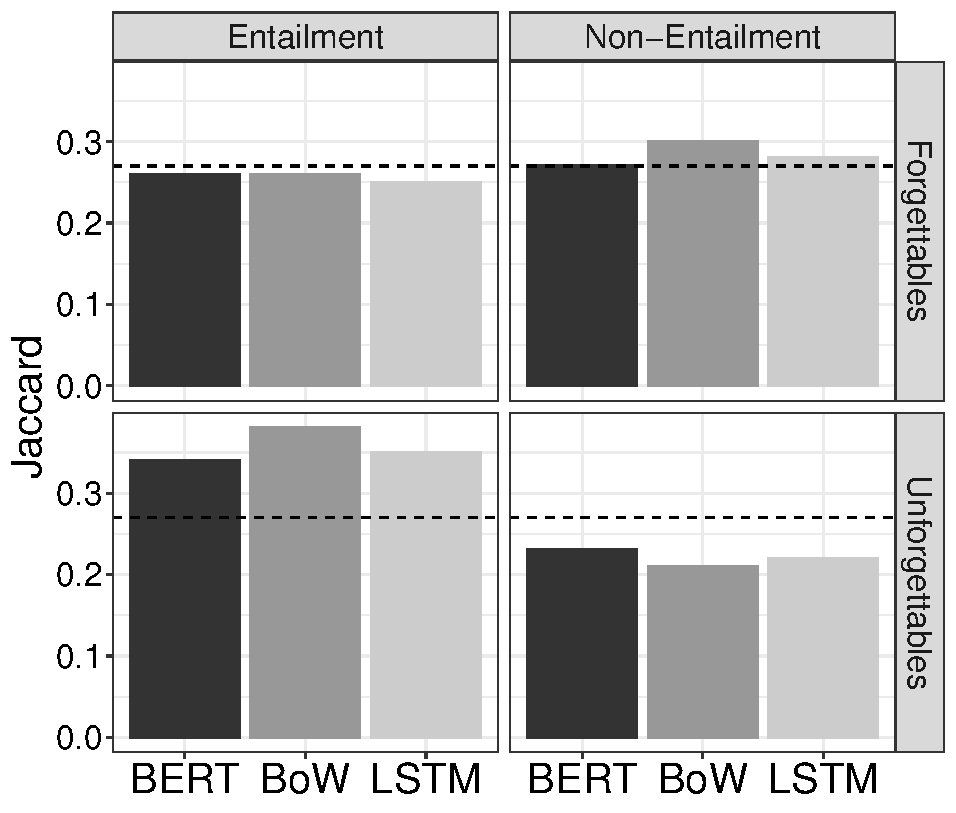
\includegraphics[scale=0.40]{figures/jaccard_by_entailment.pdf}
  \caption{Word overlap between premise and hypothesis as measured by Jaccard similarity in both forgettables and unforgettables examples. For all models, forgettable (unforgettable) examples tend to contain non-entailment (entailment) examples with higher than average (dashed line) word overlap which support their usefulness to unlearn the word overlap heuristic.}
\label{fig:wordoverlap-unforg}
\end{figure}
Fine-tuning on \flstm (line 9) is comparable to fine-tuning on \fbow (line 10) which demonstrates that both BoW and BiLSTM models learn the heuristics first.
%\textcolor{red}{This is an important sanity check as BoW models are bound to be very sensitive to the lexical overlap heuristic, while Siamese BiLSTM models do not encode known biases. It supports the notion that prior knowledge of the dataset biases is not necessary to build more robust models.}
% This shows that the choice of the weak model does not seem to matter and therefore prior knowledge about the dataset biases is not required.
We also note that while training BERT on its own forgettables (line 8) provides less improvement in robustness than on \flstm or \fbow, it does generate a significant 9.5\% increase in performance.
% We hypothesize that this is due to the smaller size of the BERT forgettables compared to BiLSTM or BoW.
% This seems to align with our hypothesis that weaker baselines capture simpler explanations in the dataset.

In Table \ref{tab:fine_mnli}, we show the performance of our method on MNLI as a function of lexical overlap, one of the main heuristic HANS was designed against. We see in particular that entailment pairs with high word overlap suffered from the fine-tuning, while non-entailment improved. This supports the intuition that the initial model relied on lexical overlap to classify pairs as entailment, and that example forgetting helps detect it (Figure \ref{fig:wordoverlap-unforg}). In Figure \ref{fig:fine_eval_baselines}, we breakdown the results of our best performing model (line 9) for the three different heuristics it was built upon. Compared to the models from \citet{clark2019dont,mahabadi2019simple}, our method does not suffer as much in the entailment class, and still provides a significant improvement for non-entailment.
% To give an example of how the various models perform, we retrieved the nearest neighbors of a given HANS example (see Appendix, Table \ref{tab:NNs}).


\paragraph{Robustness of XLNET and larger models}
% \citet{yang2019xlnet} recently introduced XLNET, a transformer-based language model outperforming BERT in standard benchmarks. We applied our evaluation procedure to XLNET and report the results in Table \ref{tab:maintable}. 
The base version of XLNET reaches 71.7\% on HANS, which is remarkably higher than BERT base version although sharing the same number of parameters\footnote{XLNET is pre-trained on more data~\citep{yang2019xlnet}.}. After fine-tuning on \flstm, we see an increase of +6.6\%; our method seems to transfer to other architectures. Perhaps more interesting is the effect of using even bigger models. A growing body of literature suggests that increasing the capacity of deep networks results in better generalization \cite{belkin2018reconciling,deepdouble}. These results usually assume no distribution shift between train and test sets. We investigate here whether robustness to the distribution shift studied in this paper may appear ``for free'' in models with a larger number of parameters. To that end, we apply our method to the ``large'' version of BERT and XLNET, \bertlarge and \xlnetlarge, which 
achieve very strong performance on the MNLI dataset~\cite{devlin2018bert,yang2019xlnet}. We see that the large versions generalize on HANS significantly better than their base counterparts (e.g. 76.1\% vs 71.7\% for XLNET, 70.6\% vs 57.9\% for BERT), confirming -- in this setting -- that larger models seem also more robust. We also observe a significant improvement in performance as a result of fine-tuning on \fbert and \fbow, supporting the applicability of the method to larger architectures. In particular, \xlnetlarge fine-tuned on \fbow shows a +7\% increase in performance, reaching 83.1\% on HANS with a maximum score of 86.8\% over 3 seeds.

\iffalse
\begin{table*}[t]
    \centering
\setlength{\tabcolsep}{4pt}
\begin{tabular}{lcrrrrrrr}
\toprule
\multirow{2}{*}{Training examples} 
&
& \multicolumn{2}{c}{lexical} & \multicolumn{2}{c}{subseq} & \multicolumn{2}{c}{const} \\
     \cmidrule(lr){3-4} \cmidrule(lr){5-6} \cmidrule(lr){7-8}
     & overall 
            & \ent            & \nent           & \ent            & \nent           & \ent             & \nent \\
\midrule
All  & 58.3     
& \bt{0.0}{96.3} & \bt{0.0}{38.4} 
& \bt{0.0}{99.6} & \bt{0.0}{4.7} 
& \bt{0.0}{99.7} & \bt{0.0}{10.6} \\
All + fine-tuning on BiLSTM forgettables & 73.6   
& \bt{0.0}{76.9} & \bt{0.0}{81.6} 
& \bt{0.0}{90.6} & \bt{0.0}{40.8} 
& \bt{0.0}{93.3} & \bt{0.0}{60.8} \\
\midrule
\newcite{mahabadi2019simple} & 66.5
& \bt{0.0}{93.5} & \bt{0.0}{61.7} 
& \bt{0.0}{96.3} & \bt{0.0}{19.2} 
& \bt{0.0}{98.4} & \bt{0.0}{30.2} \\
\newcite{clark2019dont}  & 69.2
& \bt{0.0}{67.9} & \bt{0.0}{77.4} 
& \bt{0.0}{84.3} & \bt{0.0}{44.9} 
& \bt{0.0}{81.0} & \bt{0.0}{59.6} \\
\bottomrule
\end{tabular}
\caption{Accuracy of the entailment (\ent) and non-entailment (\nent) classes on HANS for three heuristics:
    lexical overlap (lexical), subsequence overlap (subseq), and constituent overlap (const).
}
\label{tab:hans-detailed}
\end{table*}
\fi